% This file was created with tikzplotlib v0.10.1.
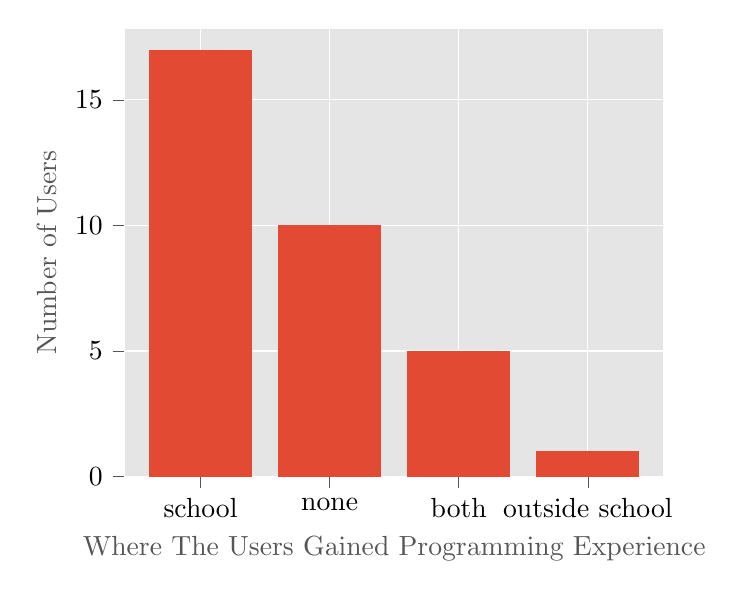
\begin{tikzpicture}

\definecolor{chocolate2267451}{RGB}{226,74,51}
\definecolor{dimgray85}{RGB}{85,85,85}
\definecolor{gainsboro229}{RGB}{229,229,229}

\begin{axis}[
axis background/.style={fill=gainsboro229},
axis line style={white},
tick align=outside,
tick pos=left,
x grid style={white},
xlabel=\textcolor{dimgray85}{Where The Users Gained Programming Experience},
xmajorgrids,
xmin=-0.59, xmax=3.59,
xtick style={color=dimgray85},
xtick={0,1,2,3},
xticklabels={school,none,both,outside school},
y grid style={white},
ylabel=\textcolor{dimgray85}{Number of Users},
ymajorgrids,
ymin=0, ymax=17.85,
ytick style={color=dimgray85}
]
\draw[draw=none,fill=chocolate2267451,very thin] (axis cs:-0.4,0) rectangle (axis cs:0.4,17);
\draw[draw=none,fill=chocolate2267451,very thin] (axis cs:0.6,0) rectangle (axis cs:1.4,10);
\draw[draw=none,fill=chocolate2267451,very thin] (axis cs:1.6,0) rectangle (axis cs:2.4,5);
\draw[draw=none,fill=chocolate2267451,very thin] (axis cs:2.6,0) rectangle (axis cs:3.4,1);
\end{axis}

\end{tikzpicture}
